\documentclass[floatsintext,man]{apa6}

\usepackage{amssymb,amsmath}
\usepackage{ifxetex,ifluatex}
\usepackage{fixltx2e} % provides \textsubscript
\ifnum 0\ifxetex 1\fi\ifluatex 1\fi=0 % if pdftex
  \usepackage[T1]{fontenc}
  \usepackage[utf8]{inputenc}
\else % if luatex or xelatex
  \ifxetex
    \usepackage{mathspec}
    \usepackage{xltxtra,xunicode}
  \else
    \usepackage{fontspec}
  \fi
  \defaultfontfeatures{Mapping=tex-text,Scale=MatchLowercase}
  \newcommand{\euro}{€}
\fi
% use upquote if available, for straight quotes in verbatim environments
\IfFileExists{upquote.sty}{\usepackage{upquote}}{}
% use microtype if available
\IfFileExists{microtype.sty}{\usepackage{microtype}}{}

% Table formatting
\usepackage{longtable, booktabs}
\usepackage{lscape}
% \usepackage[counterclockwise]{rotating}   % Landscape page setup for large tables
\usepackage{multirow}		% Table styling
\usepackage{tabularx}		% Control Column width
\usepackage[flushleft]{threeparttable}	% Allows for three part tables with a specified notes section
\usepackage{threeparttablex}            % Lets threeparttable work with longtable

% Create new environments so endfloat can handle them
% \newenvironment{ltable}
%   {\begin{landscape}\begin{center}\begin{threeparttable}}
%   {\end{threeparttable}\end{center}\end{landscape}}

\newenvironment{lltable}
  {\begin{landscape}\begin{center}\begin{ThreePartTable}}
  {\end{ThreePartTable}\end{center}\end{landscape}}




% The following enables adjusting longtable caption width to table width
% Solution found at http://golatex.de/longtable-mit-caption-so-breit-wie-die-tabelle-t15767.html
\makeatletter
\newcommand\LastLTentrywidth{1em}
\newlength\longtablewidth
\setlength{\longtablewidth}{1in}
\newcommand\getlongtablewidth{%
 \begingroup
  \ifcsname LT@\roman{LT@tables}\endcsname
  \global\longtablewidth=0pt
  \renewcommand\LT@entry[2]{\global\advance\longtablewidth by ##2\relax\gdef\LastLTentrywidth{##2}}%
  \@nameuse{LT@\roman{LT@tables}}%
  \fi
\endgroup}


\ifxetex
  \usepackage[setpagesize=false, % page size defined by xetex
              unicode=false, % unicode breaks when used with xetex
              xetex]{hyperref}
\else
  \usepackage[unicode=true]{hyperref}
\fi
\hypersetup{breaklinks=true,
            pdfauthor={},
            pdftitle={A multi-faceted, open source, measure of personality},
            colorlinks=true,
            citecolor=blue,
            urlcolor=blue,
            linkcolor=black,
            pdfborder={0 0 0}}
\urlstyle{same}  % don't use monospace font for urls

\setlength{\parindent}{0pt}
%\setlength{\parskip}{0pt plus 0pt minus 0pt}

\setlength{\emergencystretch}{3em}  % prevent overfull lines


% Manuscript styling
\captionsetup{font=singlespacing,justification=justified}
\usepackage{csquotes}
\usepackage{upgreek}

 % Line numbering
  \usepackage{lineno}
  \linenumbers


\usepackage{tikz} % Variable definition to generate author note

% fix for \tightlist problem in pandoc 1.14
\providecommand{\tightlist}{%
  \setlength{\itemsep}{0pt}\setlength{\parskip}{0pt}}

% Essential manuscript parts
  \title{A multi-faceted, open source, measure of personality}

  \shorttitle{HU instrument}


  \author{Victor Rouco\textsuperscript{1,2}, Anja Cengia\textsuperscript{3}, \& Matthias Ziegler\textsuperscript{3}}

  % \def\affdep{{"", "", ""}}%
  % \def\affcity{{"", "", ""}}%

  \affiliation{
    \vspace{0.5cm}
          \textsuperscript{1} Universitat de Barcelona\\
          \textsuperscript{2} Institut de Neurociencies Barcelona\\
          \textsuperscript{3} Humboldt Universität zu Berlin  }

  \authornote{
    Add complete departmental affiliations for each author here. Each new
    line herein must be indented, like this line.
    
    Enter author note here.
    
    Correspondence concerning this article should be addressed to Victor
    Rouco, Postal address. E-mail:
    \href{mailto:victorrouco@ub.edu}{\nolinkurl{victorrouco@ub.edu}}
  }


  \abstract{Enter abstract here. Each new line herein must be indented, like this
line.}
  \keywords{keywords \\

    \indent Word count: X
  }





\usepackage{amsthm}
\newtheorem{theorem}{Theorem}[section]
\newtheorem{lemma}{Lemma}[section]
\theoremstyle{definition}
\newtheorem{definition}{Definition}[section]
\newtheorem{corollary}{Corollary}[section]
\newtheorem{proposition}{Proposition}[section]
\theoremstyle{definition}
\newtheorem{example}{Example}[section]
\theoremstyle{definition}
\newtheorem{exercise}{Exercise}[section]
\theoremstyle{remark}
\newtheorem*{remark}{Remark}
\newtheorem*{solution}{Solution}
\begin{document}

\maketitle

\setcounter{secnumdepth}{0}



\hypertarget{introduction}{%
\section{1. Introduction}\label{introduction}}

\hypertarget{short-history-and-relevance-of-the-big-five}{%
\subsection{1.1. Short history and relevance of the Big
Five}\label{short-history-and-relevance-of-the-big-five}}

Over the last decades, the Five Factor Model as well as the Big Five
model have become widely accepted models for describing general
attributes of personality. Often the terms are even used synonymously,
which is why we will refer to the Big Five from here on. The Big Five is
a hierarchical model which describes human individual differences in
personality at the dispositional level: one of the most basic,
universal, biologically-influenced and stable layers of human
inter-individual differences in behavior, cognition and feeling (McAdams
\& Pals, 2006). Its hierarchical nature is relevant to acknowledge
behavior from the most specific (nuances), to the most broad differences
in temperament and character (dimensions), through a varying number of
mid-level personality characteristics called facets. Most of the
research concerning criterion validity of the Big Five inventories has
focused on the covariation between the Big Five dimensions and relevant
external outcomes. However, specific dispositional characteristics
captured on the facet level might be of extreme utility to provide more
complex descriptions of individuality and to predict life outcomes to a
major extent (John et al., 2014; Lounsbury, Sundstrom, Loveland, \&
Gibson, 2002; Paunonen \& Ashton, 2001). Unfortunately, the number and
nature of the facets below the Big Five and being measured by different
personality instruments is far from being consensual. In fact, different
facet level models have been proposed (XXXX). One potential reason for
this could be that many facet level models were developed after a
questionnaire version without such a level had been published. Thus, the
facets were developed as an elaboration. While this has many theoretical
advantages it also has the disadvantage of potentially limiting the
search space of possible facets. In this work we aim at maximizing this
search space and present a personality questionnaire which is broad at
the facet level, open-access, and measurement invariant across two
different cultures.

\hypertarget{a-short-history-of-the-big-five}{%
\subsection{1.2. A short history of the Big
Five}\label{a-short-history-of-the-big-five}}

Francis Galton proposed the fundamental lexical hypothesis as a ground
from where to describe interpersonal differences in personality. The
hypothesis states that every apprehended characteristic in the realm of
personality should have its place in the natural language, a corollary
derived from this first statement is that the essential features must
represent a unique word in the lexical universe of this language. Galton
himself (1884), and later Allport and Odbert (1936) and still later
Norman (1967) used English dictionaries for a systematic collection of
all adjectives which could be related to human personality
characteristics. Using exploratory factor analyses on self- and other
ratings five broad factors could repeatedly be extracted from the data.
These efforts were also replicated in different languages, such as in
German (Klages,\ldots{}), Baumgartner,\ldots{}

Cattell was one of the first researchers who systematically applied
exploratory factor analysis in order to explore personality structure.
He inspected the correlation structure of the items in the word lists of
his predecessors, finding 16 personality oblique factors, including one
factor specifically for intelligence, these factors form the 16-PF.
These 16 factors were the primary factors in a hierarchical structure
for Cattell (coetany to L.L. Thurstone and undoubtedly influenced by
him). Cattell himself viewed personality as a hierarchical structure,
containing three layers (Cattell, 1956). The second order factors
resemble the Big Five dimensions (Digman, 1990).

Different researchers followed Cattell in the study of dispositional
traits of personality. One of the most influential models was Eysenck`s
Big Three. Grounded on a strong biological basis, Eysenck`s theory
supposed a link between temperament and personality. Its structural
proposal concerned at first two big factors, named Neuroticism
vs.~Emotional stability and Extraversion vs.~Introversion. These two
dimensions were later joined by a third factor that Eysenck called
Psychoticism. This label was criticized by others who suggested that a
more appropriate term would be psychopathy (Digman, 1990). Eysenck`s big
two are still „alive`` today in the Big Five, and his third factor,
psychoticism, can be operationalized as two dimensions of the Big Five:
Agreeableness (or \ldots{}) and Conscientiousness (or \ldots{}.).

A large number of studies have focused on the problem of personality
structure resulting in a five factor solution (Fiske, 1949; Norman,
1963; Tupes \& Christal, 1961; Borgatta, 1964). Possibly the two most
widely cited works relating to the foundations of the Big Five are those
by Goldberg (\ldots{}) and McRae Costa (\ldots{}). Goldberg can be seen
as one of the first who extended research concerning the Big Five, while
McRae and Costa`s importance rests on popularizing the terminology
(OCEAN) and the development of one of the most used tools to assess
personality based on the Big Five: the NEO-PI. The Big Five dimensions
are labeled as follows: I) Extraversion vs.~Introversion. II)
Agreeableness or Friendliness. III) Conscientiousness or Achievement or
Will. IV) Emotional Stability vs.~Neuroticism. V) Openness or Intellect
or Culture.

One of the most important features of the Big Five is the fact that it
could be replicated in different languages. Research is available in
Japanese, Vietnamese, German, Spanish, Greek, (refs)\ldots{} This
finding suggests that the way human beings construe personality is at
some point universal and that its basic features are retained within the
Big Five. Another essential characteristic relies on its hierarchical
nature. The five domains are useful to retain the big picture of
personality, maximize the situation consistency and reliably assess
difficult subjects such as children. Nonetheless, each dimension is
conceptualized as a latent construct formed by more specific narrow
factors called facets, which in turn are useful to depict the impact of
personality characteristics into specific behaviors and concrete life
outcomes.

The Big Five has proven to be a valid theoretical and empirical model to
predict relevant life outcomes. Research such as Ozer and Benet-Martinez
(2006) or Roberts; Kuncel; Shiner; Caspi \& Goldberg ( 2007) has shown
that scores for the Five Dimensions (and their related facets) are able
to explain outcomes such as Academic and work performance, health,
personality disorders, political attitudes and many more. The empirical
findings linking Big Five measures to life outcomes have reinforced the
concurrent validity of the test scores interpretations. At the same
time, the broad nature of the domains has spurned research into the more
fine-grained lower order structure of facets.

\hypertarget{facet-structures}{%
\subsection{1.3. Facet Structures}\label{facet-structures}}

There are a number of models that include a facet structure below the
five broad domains. The most widely known model is the one suggested by
Costa and McCrae (XXX). Other popular models have been suggested for the
Big Five Inventory 2 (BFI-2, Soto \& John, 2017), the IPIP (JRP paper),
and the HEXACO model (XXX), which assumes six broad domains. Table 1
gives an overview of these different models listing their facets per
domain as well as some information regarding their psychometric
properties.

table 1

As shown in table 1, there are many different possibilities of facets
forming the domains. However, there is still a degree of overlap on the
facets covered by the different instruments. Soto and John (2009)
inspected the convergences between the NEO-PI-R and the first version of
the BFI, suggesting that two constructs per domain were measured at the
facet level by both inventories. The constructs defined by Soto and John
(2009) were: Assertiveness and Activity for Extraversion; Altruism and
Compliance for Agreeableness; Order and Self-Discipline for
Conscientiousness; Anxiety and Depression for Neuroticism; and
Aesthetics and Ideas for Openness. The convergence holds for the four
instruments listed in table 1, as these ten constructs are covered
within the facets for every instrument. Some of the constructs are
explicitly covered at the facet level (e.g.~Anxiety); meanwhile others
are mainly covered though the four instruments, although sometimes
implicitly (e.g.~Liveliness in HEXACO resembles the \enquote{core}
construct Activity, present in all other instruments). The reverse is
not always true, not every facet within the four instruments is covered
by the constructs proposed by Soto \& John (2008). As an example we find
Self-Consciousness, a Neuroticism facet defined by the NEO-PI-R and the
IPIP-NEO-120, which is clearly tapping at a construct different from
Anxiety or Depression.

The nomological network commonly assumed in Big Five questionnaires is
drawn from nuances through facets to domains, from more specific to more
general. Relying in domains to explain and predict behavior can benefit
from ease of interpretability. However, optimal predictions for specific
contexts can be enhanced if a more specific set of traits is used. On
the other hand, using nuances to predict behavior might yield even
stronger predictive ability (Seeboth \& Mottus, 2018), but as the number
of predictors grows the interpretations become more complex. Facets are
on a middle ground between nuances and domains, in a compromise between
specificity and sensitivity in the bandwidth-fidelity dilemma. This
narrow aggregation both satisfies the specificity of predictions to
concrete situations and environments and also enhances the ease of
interpretability when summarizing individual personality
characteristics.

Furthermore, there is a large corpus of research which points towards
facets as important criterion predictors showing incremental validity to
domains. For academic achievement, Paunonen and Ashton (2001) showed
that the facets achievement motivation and intellectual curiosity
increased the variance accounted for by college students' grades, above
and beyond its respective dimensions: Conscientiousness and Openness to
experience. Similarly, Lounsbury et al. (2002) provided evidence
regarding the facets work drive and aggression, which added an extra
12\% of explained variance over the Big Five domains on 10th grade
students' GPA. Ziegler, Danay, Schölmerich, and Bühner (2010) showed
that better performance in college grades was associated with low
gregariousness, excitement seeking and order as well as high activity,
openness to ideas and openness to values. Often different facets within
the same domain can have effects in opposite directions, partially
canceling out the predictive ability when only paying attention to the
domain score. This is the case for Openness to ideas vs.~Openness to
fantasy, as the former is related positively to academic achievement
whereas the latter is related negatively ({\textbf{???}}), resulting in
a potential masking effect on the ability of Openness predicting the
academic achievement.

As described above, facet measures often yield scores that have stronger
test-criterion correlations than their respective domain scores (e.g.,
Ziegler et al., 2012; \ldots{}). However, facet scores have also been
shown to be related to personality disorders. Thus, the combination of a
higher fidelity along with the potential clinical relevance of facet
scores might open up unique advantages for clinical research.

\hypertarget{the-big-five-and-personality-disorders}{%
\subsection{1.4. The Big Five and Personality
Disorders}\label{the-big-five-and-personality-disorders}}

Personality disorders are steadily shifting from a categorical
definition into a continua conceptualization within the clinical realm.
This process is not new for personality science history, as the subject
itself moved from a qualitatively distinct set of definitions, called
types, into a subset of continuous domains in which both normality and
extreme tendencies were moving along, named traits. In fact, the new
version of the Diagnostic and Statistical Manual of mental disorders,
DSM- V, now proposes two different ways of assessing personality
disorders: 1) A descriptive model of personality disorders in section II
which mimics the former model of assessing personality disorders and; 2)
A novel trait model that follows research on the personality scientific
domain (In section III), which conceptualizes personality disorders as
extreme tendencies located in the continuum of the Big Five domains and
facets (American Psychiatric Association, 2013; Widiger \&
Mullins-Sweatt, 2009)

This paradigm shift in clinical assessment of personality has led to the
construction of the Personality Disorder Inventory (PID-5; Krueger,
Derringer, Markon, Watson, \& Skodol, 2013), a 25-facet and
five-dimension self-report inventory, with an informant-report version
(Markon, Quilty, Bagby, \& Krueger, 2013). The big five dimensions
mirror the Big Five domains, although with a focus on the maladaptative
end of the continuum,: I) Detachment (Big Five's introversion), II)
Antagonism (absence of Big Five's Agreeableness), III) Disinhibition
(absence of Big Five's Conscientiousness), IV) Negative affect (Big
Five's Neuroticism) and V) Psychoticism (Absence of Big Five's
Openness). The PID-5 has shown satisfying evidences of criterion
validity (\ldots{}summary). However, the limited number of facets on the
PID-5 has already raised some concerns due to the low reliability when
studying developmental phenomena of personality disorders (Clercq et
al., 2014)`, and may also limit the capacity of portraying vivid
personality profiles which are suitable for explanatory purposes in the
clinical domain.

In line with what has been stated previously for academic achievement,
the examination of facets may result in an enhancement of the
specificity of assessment when looking at the nature of PDs (Clark,
2005; Samuel \& Widiger, 2008). This improvement of specificity resulted
in a predictive gain ranging from 3\% to 16\% when comparing facets to
domains predicting PD in the Reynolds and Clark (2001) study.
Furthermore, the use of facets may be of extreme utility for those PD
whose personality profile is less clear at the domain level. As Saulsman
and Page (2004) point out, Schizotypal and Obsessive-Compulsive
disorders are examples of PD which are not well covered by Big Five
domains. A reason for it may be found in a pattern inconsistency of
facets within the same dimension or in a lack of coverage for essential
characteristics of the PD. For example, aberrant cognitions are
essential characteristics of schizotypal disorder and are not covered by
some instrument's facets like the NEO-PI-R (Samuel \& Widiger, 2008;
Saulsman \& Page, 2004). Likewise, the expected high scores on warmth
and low scores on assertiveness could mask the effects of extraversion
when predicting Dependent Personality Disorder, following the
theoretical correspondence between PD and Big Five facets proposed by
Costa Jr. and Widiger (1994). Moreover, the PID-5 has prompted the
elaboration of a number of Five Factor Model Personality Disorders
(FFMPD) scales to maximize the facet coverage in relation to specific
PDs (Bagby \& Widiger, 2018).

Facet analysis and dedicated Big Five questionnaires have been used to
solve issues like those mentioned in the last paragraph. We propose to
base such research on a broader facet basis. To this end we suggest a
general instrument to cover a broad number of facets which could aim for
fine grained assessments.

\hypertarget{this-study}{%
\subsection{1.5. This study}\label{this-study}}

We present in this paper an instrument for personality assessment which
aims to cover the need for an internationally usable, open source, and
differentiated measure at the facet level. Two studies are presented,
for each one inspects the factor structure of the instrument in a
different sample drawn from a different culture (American vs.~German).
Measurement invariance across samples will be examined. Internal
consistency and test-criterion correlations will be estimated for all
scores. To sum up, the aim for this research project was to provide an
instrument that can be used in non-clinical but also in clinical
research which emphasizes the facet level of the Big Five.

\hypertarget{methods}{%
\section{2. Methods}\label{methods}}

Two different studies are presented in this work. The first study uses
sample drawn from a USA bachellor student population. The aim is to
detect and confirm a measurement model that maximizes the facet space of
the IPIP instrument. An Exploratory Factor Analysis (EFA) is used to
identify the number of facets per domain. A Confirmatory Factor Analysis
per facet is modelled in order to confirm the item - facet relationship.
Finally, an Exploratory Strucutural Equation Model (ESEM) is fitted to
integrate the measurement model of the facets with the dimensions. ESEM
is a somewhat novel method which allows the researcher to use Structural
Equation Modelling (SEM) without the need of imposing an independent
cluster solution, as its common in the CFA procedure. ESEM has gained
reputation in the personality field, where the independent cluster model
may not capture the complexity of the constructs measured (Marsh et al.,
2010).

The second sample is drawn again from a graduate student population,
albeit based in Germany. The aim for the second study is to replicate
the structure found in study one, plus assess the degree of measurement
invariance of the proposed model.

\hypertarget{study-1---us-american-sample}{%
\subsection{2. Study 1 - US-American
Sample}\label{study-1---us-american-sample}}

\hypertarget{participants}{%
\subsubsection{2.1.1. Participants}\label{participants}}

The sample consisted of 726 American undergraduate students (59.3\%
male) who participated voluntarily. The mean age was 21.6 years
(SD=5.9). Students were emailed a link to a computerized assessment
battery that included the IPIP items as well as several other tests not
reported in this paper.

At a first data preparation the data set was randomly split in two
equally sized samples. Both samples were matched in relation to missing
values, outliers and extreme values. In Sample 1 the mean age was 21.8
years (SD=6.3), in Sample 2 the mean age was 21.5 years (SD=5.6).

\hypertarget{measures.}{%
\subsection{2.1.2. Measures.}\label{measures.}}

\hypertarget{international-personality-item-pool-ipip}{%
\subsubsection{International Personality Item Pool
(IPIP)}\label{international-personality-item-pool-ipip}}

Altogether, 525 items from the \emph{International Personality Item
Pool} \emph{(IPIP)} were used to measure Neuroticism, Extraversion,
Openness (to experience), Agreeableness and Conscientiousness. The IPIP
is an open source database of personality items, which was launched in
1996, and contains over 2000 items (L. R. Goldberg et al., 2006).
Participants were asked to rate themselves on typical behaviors or
reactions on a 5-point Likert scale, ranging from 1 (\enquote{Not all
like me}) to 5 (\enquote{Very much like me}).

\hypertarget{gpa}{%
\subsubsection{GPA}\label{gpa}}

This measures academic achievement.

\hypertarget{satisfaction-with-life-swl}{%
\subsubsection{Satisfaction With Life
(SWL)}\label{satisfaction-with-life-swl}}

Scale of satisfaction with life

\hypertarget{procedure}{%
\subsection{2.1.3. Procedure}\label{procedure}}

\hypertarget{efa-with-subsample-1}{%
\subsubsection{EFA with subsample 1}\label{efa-with-subsample-1}}

To determine the number of possible facets per domain Velicer's (1976)
Minimum Average Partial (MAP) method and Horn's (1965) parallel analysis
(PA) method were employed for every domain. Based on these results an
exploratory factor analysis was calculated for each domain via Mplus
using a geomin rotation (Quelle) and a maximum likelihood estimator
(ML). The decision for the preferred number of facets per domain was
based partly on comparing model fits (CFI, RMSEA, SRMR). More
importantly though was the interpretability of the facet solution. After
all facet solutions of other personality measures were looked at to
compare it to the found facet structure. If there were important parts
missing to present the domain with regards to content, new facets would
be added afterwards.

\hypertarget{cfa-and-esem-with-subsample-2}{%
\subsubsection{CFA and ESEM with subsample
2}\label{cfa-and-esem-with-subsample-2}}

To confirm the structure of facets the EFAs delivered, multiple
confirmatory factor analyses were calculated via Mplus. In a first step
measurement models were estimated for each of the facets. To obtain
balance between the facets, the items were reduced to five per facet
based on item content and loading pattern in a second step, afterwards
the estimations for the measurement models on facet levels were
repeated. For both steps estimators were WLSMV (weighted least squares
adjusted for means and variances). Aim was to ensure an optimal breadth
and sufficient reliability. In a final model, all five domain structural
models were integrated using exploratory structural equation modeling
(ESEM) (Asparouhov \& Muthén, 2009). Marsh et al. (2010) could show that
ESEM fits personality data better and results in substantially more
differentiated factors than it would using CFA, while using an EFA
measurement model with rotations in a structural equation model. All
facets were able to load on all domains. If there would show up facets
that do not significantly load on the intended domain, this facets would
get eliminated subsequently. The estimators used were ML (maximum
likelihood), factor scores were used as indicators and the rotation was
oblique (using Geomin). Model fit was determined based on the guide
lines by Hu and Bentler (1999) as well as Beauducel and Wittmann (2005).
Consequently, to consider a good fit of a proposed model, the
Comparative Fit Index (CFI) should be at or over .95, the standardized
root mean squared residual (SRMR) smaller than .08 and the root mean
square error of approximation (RMSEA) smaller than .06.

\hypertarget{criterion-validity-evidence}{%
\subsubsection{Criterion validity
evidence}\label{criterion-validity-evidence}}

To examine the nomological structure of the facets and domains to
external constructs like life satisfaction and education, correlations
and multiple regression were computed.

\hypertarget{results}{%
\subsection{2.2. Results}\label{results}}

\hypertarget{results-of-efa}{%
\subsubsection{Results of EFA}\label{results-of-efa}}

In \emph{Table 2} you can see model fits for the chosen facet model for
each domain as well as Eigenvalues and results from MAP and PA test.

To ensure that each facet is homogeneous and therefore, to reduce the
risk of cross domain loadings, items with factor loadings less than .30
were eliminated. This was only done when item content was also judged as
being non-central to the domain in question (Ziegler, 2014).

According to that Agreeableness consists of eight facets after two
facets were eliminated due to weakly loading and inconsistent items. The
remaining facets are named Appreciation, Integrity, Low Competitiveness,
Readiness to Give Feedback, Search for Support, Good Faith, Genuineness
and Altruism.

Conscientiousness consists of nine facets after one facet with item
factor loadings less than .30 was excluded, which are named: Dominance,
Persistence, Self-discipline, Task planning, Goal orientation,
Carefulness, Orderliness, Wish to work to capacity and Productivity.

Extraversion comprises of nine facets, after a new facet (Energy) was
added. The original model with eight facets did not explain the physical
part of Extraversion very well. The facets are Sociability, Readiness to
take risks, Wish for affiliation, Positive attitude, Forcefulness,
Communicativeness, Humor, Conviviality and Energy.

Neuroticism (here interpreted in the way of emotional stability)
consists of seven facets. One facet was dropped due to poor
interpretability, and was therefore not included in the subsequent
analyses. The final set of facets are named Equanimity, Confidence,
Carefreeness, Mental balance, Drive, Emotional robustness and
Self-attention.

Openness to experience comprises of nine facets. One facet was
identified as a method factor and eliminated, because it solely
contained negatively formulated items and no coherent underlying trait
could be identified. Furthermore another facet (Intellect) was added,
because the remaining facets lacked an intellectual content. The facets
of Openness are named Creativity, Wish for variety, Open-mindedness,
Interest in reading, Artistic interests, Wish to analyze, Willingness to
learn, Sensitivity and Intellect.

The items to each facet are listed in the appendix (A).

\hypertarget{results-of-cfa-and-esem.}{%
\subsubsection{Results of CFA and
ESEM.}\label{results-of-cfa-and-esem.}}

All measurement models for the facets were fitting well, results can be
found in \emph{Table 3}.

Table 3

The exploratory structural equation model (ESEM) of the final model with
all five domains fits well with CFI = .87, RMSEA = .072, SRMR = .036. As
you can see in \emph{Table 4} nearly all facets load significantly on
their intended domain, but sometimes have loadings on other domains
also, which are conform with the theory and the facet content.

\hypertarget{study-2-german-translation}{%
\section{Study 2 -- German
Translation}\label{study-2-german-translation}}

\hypertarget{methods-1}{%
\subsection{Methods}\label{methods-1}}

\hypertarget{participants-1}{%
\subsubsection{Participants}\label{participants-1}}

The representative sample consisted of 387 German speakers (49.1\% male)
with a mean age of 45.6 years (SD=17.5).

\hypertarget{measures}{%
\subsubsection{Measures}\label{measures}}

The five items per facet derived from Study 1 were translated and
back-translated by bilingual experts, creating a German version of the
measure used there.

\hypertarget{procedure-1}{%
\subsection{Procedure}\label{procedure-1}}

\hypertarget{step-1-examining-the-structure.}{%
\subsubsection{Step 1 -- Examining the
structure.}\label{step-1-examining-the-structure.}}

To check the facet structure Study 1 delivered, multiple confirmatory
factor analyses were calculated via Mplus following an analogue
procedure to Study 1. First, measurement models were estimated for all
facets, estimator was WLSMV. Model fit was determined based on the guide
lines as before. In a final model, all five domain structural models
were integrated using again exploratory structural equation modeling
(ESEM).

\hypertarget{step-2-testing-for-measurement-invariance.}{%
\subsubsection{Step 2 -- Testing for measurement
invariance.}\label{step-2-testing-for-measurement-invariance.}}

In a next step, measurement invariance between German and US samples was
examined. We followed the procedure suggested by Sass (2011) and tested
configural, factorial and strong factorial invariance. The cutoffs
suggested by Chen (2007) were applied to compare model fits. According
to this configural measurement invariance can be assumed when the same
item is associated with the same factor in each domain, while the factor
loadings can differ. If the factor loadings of each item would not
differ between the samples, factorial measurement invariance can be
assumed. Strong factorial measurement invariance can be assumed when on
top of that the intercepts of each item are equal. The limit to
factorial measurement invariance was set to \(\Delta\) CFI \textless{}
.01, \(\Delta\) RMSEA \textless{} .015 and \(\Delta\) SRMR \textless{}
.03, at which the limit to strong factorial measurement invariance was
set to \(\Delta\) CFI \textless{} .01, \(\Delta\) RMSEA \textless{}
.015, \(\Delta\) SRMR \textless{} .01 (Chen, 2007).

\hypertarget{results-1}{%
\subsection{Results}\label{results-1}}

\hypertarget{results-of-cfa}{%
\subsubsection{Results of CFA}\label{results-of-cfa}}

The measurement models of the American sample were replicated for the
reduced number of item per facet. Model fits can be seen in Table 4. The
ESEM with all five domains fits well with CFI = .82, RMSEA = .078, SRMR
= .044. Table 5 shows the ESEM factor loadings for the German sample.
All facets load significantly on their intended domain but can have
loadings on other domains as well.

\hypertarget{results-of-mi}{%
\subsection{Results of MI}\label{results-of-mi}}

For analyzing the measurement invariance the latest facet model
structure (with additional facets) was taken. The results are shown in
Table 6. Configural measurement invariance is assumed for the facets
Appreciation of others, Superiority/Grandiosity, Need to be liked,
Crybabiness, Manipulation, Altruism (facets of Agreeableness),
Perseverance, Task Planning, Goal-orientation/Achievement striving,
Preferred Load, Procrastination (facets of Conscientiousness),
Assertiveness, Sociability/Gregariousness, Activity (facets of
Extraversion), Irritability, Self-serving Attention (facets of
Neuroticism), Self-attributed Inginuity, Openness to actions and
activities, Openmindedness/Judgement, Love of Learning, Openness to
feelings and Intellect (facets of Openness).

Factorial measurement invariance is assumed for the facets Meanness,
Trust (facets of Agreeableness), Control of others, Lack of (Self-)
Control, Deliberation/Caution, Lack of Tidiness/Order (facets of
Conscientiousness), Sensation Seeking, Reclusiveness, Emotionality,
Humor (facets of Extraversion), Depression, Anxiety, Self-assuredness,
Lethargia, Sentimentality (facets of Neuroticism), Openness to reading,
Openness to arts and Need for cognition (facets of Openness).

The only facet with strong factorial measurement invariance is Shyness,
a facet of Extraversion

\newpage

\hypertarget{references}{%
\section{References}\label{references}}

\begingroup
\setlength{\parindent}{-0.5in}
\setlength{\leftskip}{0.5in}

\hypertarget{refs}{}
\leavevmode\hypertarget{ref-Bagby2018}{}%
Bagby, R. M., \& Widiger, T. A. (2018). Five factor model personality
disorder scales: An introduction to a special section on assessment of
maladaptive variants of the five factor model. \emph{Psychological
Assessment}, \emph{30}(1), 1--9.
doi:\href{https://doi.org/10.1037/pas0000523}{10.1037/pas0000523}

\leavevmode\hypertarget{ref-Clark2005}{}%
Clark, L. A. (2005). Temperament as a unifying basis for personality and
psychopathology. \emph{Journal of Abnormal Psychology}, \emph{114}(4),
505--521.
doi:\href{https://doi.org/10.1037/0021-843X.114.4.505}{10.1037/0021-843X.114.4.505}

\leavevmode\hypertarget{ref-Widiger1994}{}%
Costa Jr., P. T., \& Widiger, T. A. (1994). A description of the
DSM-III-R and DSM-IV personality disorders with the five-factor model of
personality. \emph{Personality Disorders and the Five-Factor Model of
Personality.}, (January), 41--56.
doi:\href{https://doi.org/10.1037/10140-003}{10.1037/10140-003}

\leavevmode\hypertarget{ref-Ziegler2014}{}%
John, O. P., Hampson, S. E., Goldberg, L. R., Johnson, J. A., Eber, H.
W., Hogan, R., \ldots{} Digman, J. M. (2014). The basic level in
personality - trait hierarchies:Studies of trait use and accessibility
in different contexts. \emph{Journal of Research in Personality},
\emph{20}(1), 411--418.
doi:\href{https://doi.org/10.1016/j.lindif.2013.10.008}{10.1016/j.lindif.2013.10.008}

\leavevmode\hypertarget{ref-Lounsbury2002}{}%
Lounsbury, J. W., Sundstrom, E., Loveland, J. L., \& Gibson, L. W.
(2002). Broad versus narrow personality traits in predicting academic
performance of adolescents. \emph{Learning and Individual Differences},
\emph{14}(1), 67--77.
doi:\href{https://doi.org/10.1016/j.lindif.2003.08.001}{10.1016/j.lindif.2003.08.001}

\leavevmode\hypertarget{ref-Marsh2010}{}%
Marsh, H. W., Lüdtke, O., Muthén, B., Asparouhov, T., Morin, A. J.,
Trautwein, U., \& Nagengast, B. (2010). A New Look at the Big Five
Factor Structure Through Exploratory Structural Equation Modeling.
\emph{Psychological Assessment}, \emph{22}(3), 471--491.
doi:\href{https://doi.org/10.1037/a0019227}{10.1037/a0019227}

\leavevmode\hypertarget{ref-McAdams2006a}{}%
McAdams, D. P., \& Pals, J. L. (2006). A new Big Five: Fundamental
principles for an integrative science of personality. \emph{American
Psychologist}, \emph{61}(3), 204--217.
doi:\href{https://doi.org/10.1037/0003-066X.61.3.204}{10.1037/0003-066X.61.3.204}

\leavevmode\hypertarget{ref-Paunonen2001}{}%
Paunonen, S. V., \& Ashton, M. C. (2001). Big Five Predictors of
Academic Achievement. \emph{Journal of Research in Personality},
\emph{35}(1), 78--90.
doi:\href{https://doi.org/10.1006/jrpe.2000.2309}{10.1006/jrpe.2000.2309}

\leavevmode\hypertarget{ref-ClarkReynolds2001}{}%
Reynolds, S. K., \& Clark, L. A. (2001). Predicting dimensions of
personality disorder from domains and facets of the Five-Factor Model.
\emph{Journal of Personality}, \emph{69}(2), 199--222.
doi:\href{https://doi.org/10.1111/1467-6494.00142}{10.1111/1467-6494.00142}

\leavevmode\hypertarget{ref-SamuelWidiger2008}{}%
Samuel, D. B., \& Widiger, T. A. (2008). A meta-analytic review of the
relationships between the five-factor model and DSM-IV-TR personality
disorders: A facet level analysis. \emph{Clinical Psychology Review},
\emph{28}(8), 1326--1342.
doi:\href{https://doi.org/10.1016/j.cpr.2008.07.002}{10.1016/j.cpr.2008.07.002}

\leavevmode\hypertarget{ref-SaulsmanPage2004}{}%
Saulsman, L. M., \& Page, A. C. (2004). The five-factor model and
personality disorder empirical literature: A meta-analytic review.
\emph{Clinical Psychology Review}, \emph{23}(8), 1055--1085.
doi:\href{https://doi.org/10.1016/j.cpr.2002.09.001}{10.1016/j.cpr.2002.09.001}

\leavevmode\hypertarget{ref-SotoJohn2009}{}%
Soto, C. J., \& John, O. P. (2009). Ten facet scales for the Big Five
Inventory: Convergence with NEO PI-R facets, self-peer agreement, and
discriminant validity. \emph{Journal of Research in Personality},
\emph{43}(1), 84--90.
doi:\href{https://doi.org/10.1016/j.jrp.2008.10.002}{10.1016/j.jrp.2008.10.002}

\leavevmode\hypertarget{ref-Ziegler2010}{}%
Ziegler, M., Danay, E., Schölmerich, F., \& Bühner, M. (2010).
Predicting Academic Success with the Big 5 Rated from Different Points
of View: Self-Rated, Other Rated and Faked. \emph{European Journal of
Personality}, \emph{24}(July 2010), 341--355.
doi:\href{https://doi.org/10.1002/per}{10.1002/per}

\endgroup





  \clearpage
  \makeatletter
  \efloat@restorefloats
  \makeatother
  
  
\begin{appendix}
\section{}
Appendix

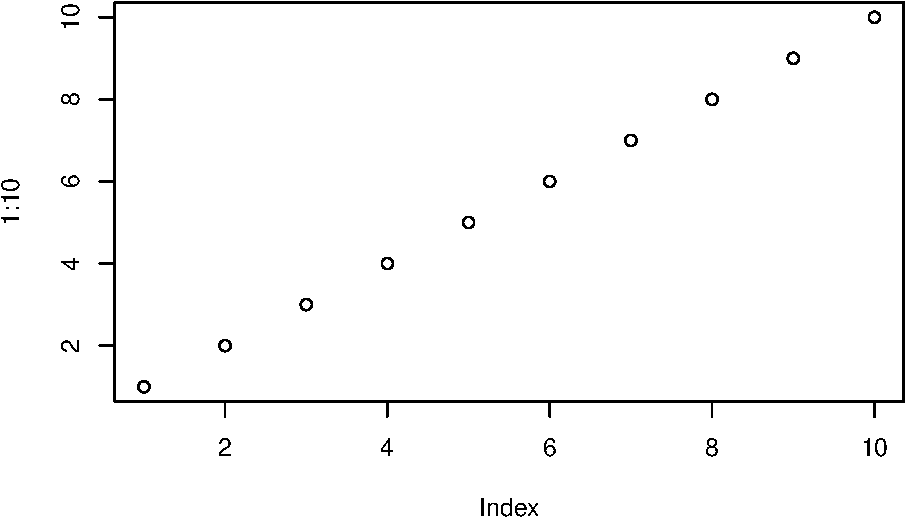
\includegraphics{IPIP_draft_files/figure-latex/unnamed-chunk-2-1.pdf}
\end{appendix}

\end{document}
